% filename GenericSettings.Rnw 



% filename Regression001.Rnw 

%\setcounter{chapter}{} 
\chapter{LURN\ldots{} To Perform Regression Analyses} 
\label{Regression} 
 
 
% filename Regression002.Rnw 


% filename Regression003.Rnw 

 
This chapter presents the most basic regression models. To really get the most out of \R{} and regression techniques (such as those taught in second or later statistics courses) you will need to look for guidance from a suitable textbook, many of which incorporate use of \R{} as the preferred software tool. 
 
\section{Data and suitable exploratory graphs} 
 
The easiest way to fit regression models is using data that are contained in a \Rclass{data.frame}. This means we can use the \Rcmd{attach} command to get at the separate components if we need them. An alternative is to have direct access to each variable independently within our current workspace. For neatness, I prefer to keep data in the \Rclass{data.frame} format. 
 
We can use the \Robject{air quality} data described in Chapter~\ref{SimpleGraphs}. Recall that it is available from your current workspace as it is contained within the \Rpackage{datasets} package. Typing 
% filename Regression004.Rnw 

\begin{Schunk}
\begin{Sinput}
> data(airquality) 
\end{Sinput}
\end{Schunk}
% filename Regression005.Rnw 

will make the data explicitly available to you in your current \R{} workspace. 
 
We can look for relationships among the variables within this data set using the techniques described in Chapter~\ref{SimpleGraphs}. Note in particular the scatter plot matrix presented in Exhibit~\ref{AirQualityScatterPlotMatrix}. 
 
 
 
\section{The simple regression model} 
 
To obtain the equation for a straight line relationship of the form \begin{equation} 
y=\alpha+\beta{}x +\varepsilon 
\end{equation} we use the \Rcmd{lm} command. The first argument for this command is a \Rclass{formula}{} which is the main component of any \Rcmd{lm} command you issue. It is of the form \code{y\textasciitilde{}x} where the $y$ is the response variable and the $x$ is the predictor variable. We will see how to modify the right hand side of the \Rclass{formula} in subsequent sections. The $\varepsilon$ is the error term for our model; we look at that aspect more in Section~\ref{RegValid}    below.  

\Blind{The above equation is a simpler version than you will see in many textbooks. You might see a subscript on the $y$, $x$, and $\varepsilon$ when referring to individual observations, but when we refer to the set of response values and the set of predictor values, we are usually thinking of them as vectors; as such, the notation above really should indicate that $y$, $x$, and $\varepsilon$ are vectors. A bold face is often used for vectors and matrices or sometimes vectors are underscored. This additional notation is not used in the current context.}


A second common argument is the \Rarg{data} statement. This means that the model formula can be stated using variable names from within the \Rclass{data.frame} mentioned in the \Rarg{data} statement. Models to explain the amount of \Robject{Ozone} using \Robject{Wind} and subsequently \Robject{Temp} are as follows. 
% filename Regression006.Rnw 

\begin{Schunk}
\begin{Sinput}
> Ozone.lm1 = lm(Ozone~Wind, data=airquality) 
> Ozone.lm1 
\end{Sinput}
\begin{Soutput}

Call:
lm(formula = Ozone ~ Wind, data = airquality)

Coefficients:
(Intercept)         Wind  
      96.87        -5.55  
\end{Soutput}
\begin{Sinput}
> summary(Ozone.lm1) 
\end{Sinput}
\begin{Soutput}

Call:
lm(formula = Ozone ~ Wind, data = airquality)

Residuals:
   Min     1Q Median     3Q    Max 
-51.57 -18.85  -4.87  15.23  90.00 

Coefficients:
            Estimate Std. Error t value Pr(>|t|)    
(Intercept)    96.87       7.24   13.38  < 2e-16 ***
Wind           -5.55       0.69   -8.04  9.3e-13 ***
---
Signif. codes:  
0 '***' 0.001 '**' 0.01 '*' 0.05 '.' 0.1 ' ' 1

Residual standard error: 26.5 on 114 degrees of freedom
  (37 observations deleted due to missingness)
Multiple R-squared:  0.362,	Adjusted R-squared:  0.356 
F-statistic: 64.6 on 1 and 114 DF,  p-value: 9.27e-13
\end{Soutput}
\begin{Sinput}
> anova(Ozone.lm1) 
\end{Sinput}
\begin{Soutput}
Analysis of Variance Table

Response: Ozone
           Df Sum Sq Mean Sq F value  Pr(>F)    
Wind        1  45284   45284    64.6 9.3e-13 ***
Residuals 114  79859     701                    
---
Signif. codes:  
0 '***' 0.001 '**' 0.01 '*' 0.05 '.' 0.1 ' ' 1
\end{Soutput}
\begin{Sinput}
> Ozone.lm2 = lm(Ozone~Temp, data=airquality) 
> summary(Ozone.lm2) 
\end{Sinput}
\begin{Soutput}

Call:
lm(formula = Ozone ~ Temp, data = airquality)

Residuals:
   Min     1Q Median     3Q    Max 
-40.73 -17.41  -0.59  11.31 118.27 

Coefficients:
            Estimate Std. Error t value Pr(>|t|)    
(Intercept) -146.995     18.287   -8.04  9.4e-13 ***
Temp           2.429      0.233   10.42  < 2e-16 ***
---
Signif. codes:  
0 '***' 0.001 '**' 0.01 '*' 0.05 '.' 0.1 ' ' 1

Residual standard error: 23.7 on 114 degrees of freedom
  (37 observations deleted due to missingness)
Multiple R-squared:  0.488,	Adjusted R-squared:  0.483 
F-statistic:  109 on 1 and 114 DF,  p-value: <2e-16
\end{Soutput}
\begin{Sinput}
> anova(Ozone.lm2) 
\end{Sinput}
\begin{Soutput}
Analysis of Variance Table

Response: Ozone
           Df Sum Sq Mean Sq F value Pr(>F)    
Temp        1  61033   61033     109 <2e-16 ***
Residuals 114  64110     562                   
---
Signif. codes:  
0 '***' 0.001 '**' 0.01 '*' 0.05 '.' 0.1 ' ' 1
\end{Soutput}
\end{Schunk}
% filename Regression007.Rnw 

There are very good reasons for creating the new objects in this example. Aside from the use of the \Rcmd{summary} method and \Rcmd{anova} command to extract more useful information about the model, we will refer back to the object using other commands in subsequent sections of this chapter. It also means we can investigate the model object, and extract some quantities on their own. For example, it's common to want to extract the $R^2$ for a model. We can't do this from the model object itself, but we can from the \Rcmd{summary} of the model. 
% filename Regression008.Rnw 

\begin{Schunk}
\begin{Sinput}
> names(Ozone.lm1) 
\end{Sinput}
\begin{Soutput}
 [1] "coefficients"  "residuals"     "effects"      
 [4] "rank"          "fitted.values" "assign"       
 [7] "qr"            "df.residual"   "na.action"    
[10] "xlevels"       "call"          "terms"        
[13] "model"        
\end{Soutput}
\begin{Sinput}
> names(summary(Ozone.lm1)) 
\end{Sinput}
\begin{Soutput}
 [1] "call"          "terms"         "residuals"    
 [4] "coefficients"  "aliased"       "sigma"        
 [7] "df"            "r.squared"     "adj.r.squared"
[10] "fstatistic"    "cov.unscaled"  "na.action"    
\end{Soutput}
\begin{Sinput}
> summary(Ozone.lm1)$r.squared 
\end{Sinput}
\begin{Soutput}
[1] 0.3619
\end{Soutput}
\end{Schunk}
% filename Regression009.Rnw 

 
 
 
\section{Presenting the straight line model's suitability in a graph} 
\label{AddFittedLine} 
 
Adding a fitted line to the scatter plot when a simple relationship has been fitted is actually a very simple task. Note that when we saw the outcome of the simple model above, we obtained just the intercept and slope coefficient values until we employed the \Rcmd{summary} method to extract more useful information. These two values will be used by the \Rcmd{abline} function to add the straight line to an existing plot. See Exhibit~\ref{RegLineAdded} for example. 
\begin{exhibit} 
\begin{center} 
\caption{Two simple regressions with the straight line added onto the scatter plots.} 
\label{RegLineAdded} 
% filename Regression010.Rnw 

\begin{Schunk}
\begin{Sinput}
> attach(airquality) 
> plot(Wind, Ozone) 
> abline(Ozone.lm1) 
\end{Sinput}

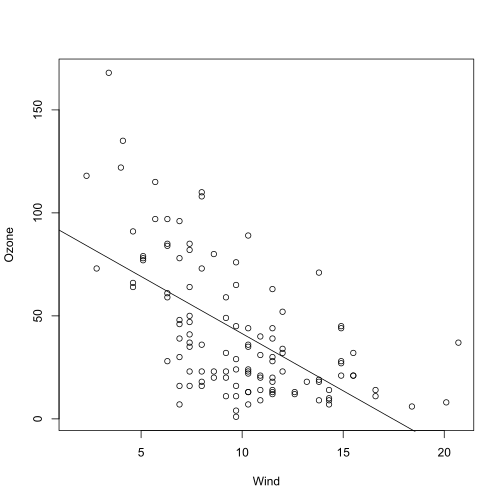
\includegraphics[width=0.7\textwidth]{figures/RegressionOzoneWindWithLine-1} \end{Schunk}
% filename Regression012.Rnw 

\begin{Schunk}
\begin{Sinput}
> plot(Temp, Ozone) 
> abline(Ozone.lm2) 
\end{Sinput}

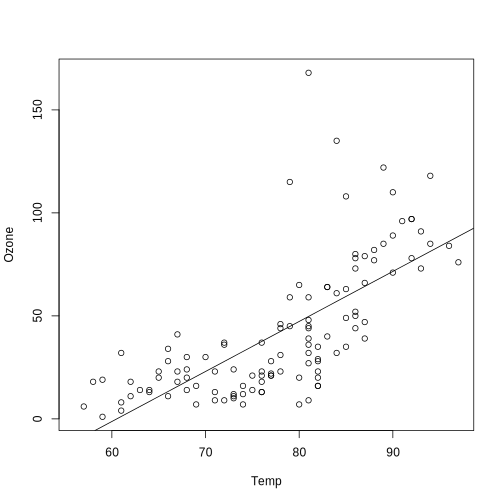
\includegraphics[width=0.7\textwidth]{figures/RegressionOzoneTempWithLine-1} \begin{Sinput}
> detach(airquality) 
\end{Sinput}
\end{Schunk}
% filename Regression013.Rnw 

\end{center} 
\end{exhibit} 
 
We can see from these graphs that our straight line model might be appropriate for explaining \Robject{Ozone} using \Robject{Temp} as the predictor, but that the straight line model using \Robject{Wind} as the predictor is not a good idea as there is fairly obvious curvature in the relationship. As it happens neither of these models are perfect and more work is required. 
 
\section{Model validation using diagnostic plots} 
\label{RegValid}  
 
\R{} has many useful built-in methods for doing common tasks efficiently. Obtaining residual plots for a model is a great example. The \Rcmd{plot} command acts on a \Rclass{lm} object by generating a series of plots. The most commonly used of these plots are the plot of residuals vs the fitted values and the normal probability plot of residuals. These plots are generated by many statistical applications but the other two presented by default in \R{} are not always given by other programs. 
\R{} also provides a Scale-Location plot of the square root of the absolute value of residuals against the fitted values, and a plot of residuals against the leverages. These approaches for diagnosing problems in a regression model are seldom taught in introductory statistics courses.  
The scale vs location plot is another means of determining if the residuals have constant variance. Leverage is a measure of how much influence an observation has on determining the model. A rule of thumb says that a leverage of more than twice the average leverage is a problem. 
 
The diagnostic plots for the inadequate model for \Robject{Ozone} being predicted by a linear function of \Robject{Wind} are presented in Exhibit~\ref{OzoneWindResidPlots}. 
\begin{exhibit} 
\begin{center} 
\caption{Residual plots for the simple regression using Wind to predict the Ozone level.} 
\label{OzoneWindResidPlots} 
% filename Regression014.Rnw 

\begin{Schunk}
\begin{Sinput}
> par(mfrow=c(2,2)) 
> plot(Ozone.lm1) 
\end{Sinput}

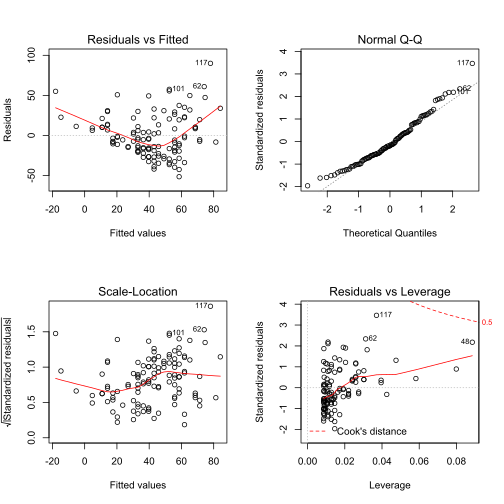
\includegraphics[width=0.7\textwidth]{figures/RegressionOzoneWindResidPlots-1} \end{Schunk}
% filename Regression015.Rnw 

\end{center} 
\end{exhibit} 
These plots are enhanced by \R{} to add more information than the basic user is familiar with. Additional lines are added to three of the plots to assist in diagnosing problems. We can see from this plot that the model is inadequate as there is a nonlinear relationship between the response and predictor, and further that the residuals might not have very constant variance. 

\Blind{There are non-graphical substitutes for the standard residuals analysis graphs that show the presence of non-constant variance;  they are seldom taught as part of the standard introduction to regression analysis. A formal hypothesis test for non-constant variance can be conducted using either the Breusch-Pagan test found using the \Rcmd{bptest} function, the Goldfeld-Quandt test found using the \Rcmd{gqtest} function, both from the \Rpkg{lmtest} package, or the Non-constant Variance test found using the \Rcmd{ncvTest} from the \Rpkg{car} package. These tests are simple to use if you are comfortable with hypothesis testing, but you will need to have the corresponding add-on package installed before proceeding.}
 
It might be easier to extract just the information we want, so we can build simpler plots ourselves. We need to find the residuals, fitted values and leverages for the model. These are found using the \Rcmd{resid}, \Rcmd{fitted}, and \Rcmd{hatvalues} commands respectively. 
% filename Regression016.Rnw 

\begin{Schunk}
\begin{Sinput}
> Ozone.resid1 = resid(Ozone.lm1) 
> Ozone.fitted1 = fitted(Ozone.lm1) 
> Ozone.lev1 = hatvalues(Ozone.lm1) 
\end{Sinput}
\end{Schunk}
% filename Regression017.Rnw 

The various plots can be constructed using the \Rcmd{plot}, and \Rcmd{qqnorm} commands as needed, but if we want the information on the leverages in text form we will need to do tasks like 
% filename Regression018.Rnw 

\begin{Schunk}
\begin{Sinput}
> mean(Ozone.lev1) 
\end{Sinput}
\begin{Soutput}
[1] 0.01724
\end{Soutput}
\begin{Sinput}
> max(Ozone.lev1) 
\end{Sinput}
\begin{Soutput}
[1] 0.08854
\end{Soutput}
\begin{Sinput}
> Ozone.lev1[Ozone.lev1>2*mean(Ozone.lev1)] 
\end{Sinput}
\begin{Soutput}
      9      18      22      48     117     121     126 
0.07994 0.05822 0.03951 0.08854 0.03703 0.04753 0.04256 
    148 
0.03951 
\end{Soutput}
\end{Schunk}
% filename Regression019.Rnw 

The last command in this block has printed out the 8 observations that have excess leverage on this model. We should probably see if these are days that had extremely high wind. This is not done as this model has already been shown to be poor at explaining the amount of \Robject{Ozone} in the atmosphere. 
 
 
\section{Polynomial regression models} 
\label{PolyReg} 
 
Given the obvious curvature in the relationship between \Robject{Ozone} and \Robject{Wind} appears monotonic, we can probably try both transforming the variables, and polynomial regression to explain the relationship. We take advantage of the  
fact that \R{} has an in-built way of producing polynomial terms for insertion into models, and use the \Rcmd{poly} function in this instance. This command needs to know which variable to work with and the degree of the polynomial desired. For example, to fit the quadratic model we would use the commands 
% filename Regression020.Rnw 

\begin{Schunk}
\begin{Sinput}
> Ozone.poly2 = lm(Ozone~poly(Wind,2, raw=TRUE), data=airquality) 
> summary(Ozone.poly2) 
\end{Sinput}
\begin{Soutput}

Call:
lm(formula = Ozone ~ poly(Wind, 2, raw = TRUE), data = airquality)

Residuals:
   Min     1Q Median     3Q    Max 
-52.29 -16.00  -4.66  12.44  64.04 

Coefficients:
                           Estimate Std. Error t value
(Intercept)                 162.572     14.185   11.46
poly(Wind, 2, raw = TRUE)1  -19.444      2.735   -7.11
poly(Wind, 2, raw = TRUE)2    0.649      0.124    5.22
                           Pr(>|t|)    
(Intercept)                 < 2e-16 ***
poly(Wind, 2, raw = TRUE)1  1.1e-10 ***
poly(Wind, 2, raw = TRUE)2  8.3e-07 ***
---
Signif. codes:  
0 '***' 0.001 '**' 0.01 '*' 0.05 '.' 0.1 ' ' 1

Residual standard error: 23.9 on 113 degrees of freedom
  (37 observations deleted due to missingness)
Multiple R-squared:  0.486,	Adjusted R-squared:  0.477 
F-statistic: 53.4 on 2 and 113 DF,  p-value: <2e-16
\end{Soutput}
\end{Schunk}
% filename Regression021.Rnw 

Note that in order to obtain a model with the correct coefficients for the polynomial terms in the model, we need to use the \Rarg{raw} argument, setting it to \code{TRUE}.  
 
We usually justify the use of a quadratic form by determining there is no practical benefit in making the model more complicated. To do this, we need to investigate the model for the cubic form of the relationship using 
% filename Regression022.Rnw 

\begin{Schunk}
\begin{Sinput}
> Ozone.poly3 = lm(Ozone~poly(Wind,3, raw=TRUE), data=airquality) 
\end{Sinput}
\end{Schunk}
% filename Regression023.Rnw 

Rather than continuously investigate the summaries of the various models, we can employ the \Rcmd{anova} command to compare the models.  
% filename Regression024.Rnw 

\begin{Schunk}
\begin{Sinput}
> anova(Ozone.lm1, Ozone.poly2, Ozone.poly3) 
\end{Sinput}
\begin{Soutput}
Analysis of Variance Table

Model 1: Ozone ~ Wind
Model 2: Ozone ~ poly(Wind, 2, raw = TRUE)
Model 3: Ozone ~ poly(Wind, 3, raw = TRUE)
  Res.Df   RSS Df Sum of Sq     F  Pr(>F)    
1    114 79859                               
2    113 64360  1     15499 27.62 7.1e-07 ***
3    112 62858  1      1502  2.68     0.1    
---
Signif. codes:  
0 '***' 0.001 '**' 0.01 '*' 0.05 '.' 0.1 ' ' 1
\end{Soutput}
\end{Schunk}
% filename Regression025.Rnw 

We can compare all three models created thus far because they are a series of nested models. We could not include the model using \Robject{Temp} as the predictor in this command for example. 
 
On the basis of the output from our \Rcmd{anova} command, we might assume that the quadratic form was sufficient to explain the relationship between \Robject{Ozone} and \Robject{Wind} because there is little to be gained by adding the cubic term to our model. Validation of the chosen model via the residual analysis is suggested as a next step. 
 
\section{Presenting the polynomial model's suitability in a graph} 
 
The \Rcmd{abline} command demonstrated earlier is only useful for straight lines. We have seen that the quadratic function is better at explaining the relationship between \Robject{Ozone} and \Robject{Wind}. One solution is to store the fitted values from this model and plot them against the \Robject{Wind} variable, but this will only show the series of points not a smooth curve.  
% filename Regression026.Rnw 

\begin{Schunk}
\begin{Sinput}
> plot(Ozone~Wind, data=airquality) 
> points(airquality$Wind[!is.na(airquality$Ozone)], fitted(Ozone.poly2), col=2) 
\end{Sinput}

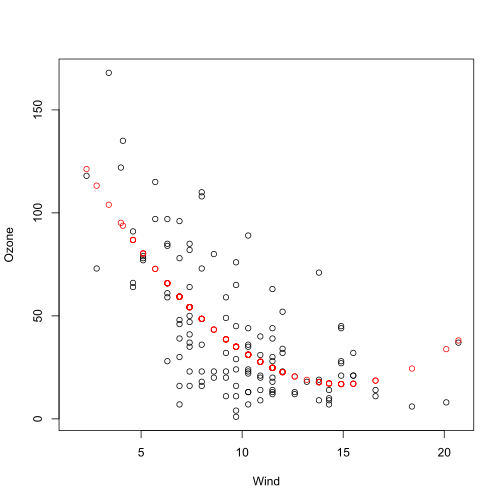
\includegraphics[width=0.7\textwidth]{figures/RegressionQuadAddPoints-1} \end{Schunk}
% filename Regression027.Rnw 

 
Note that the \Rcmd{points} command used here includes the \Rarg{col} argument to change the colour of the points to red --- the second colour in the list of colours.  
 
Also note that there are missing values in the records for \Robject{Ozone}. The fitted values from the model are only calculated for the observations where \Robject{Ozone} was recorded, so we have employed the \Rcmd{!} logical operator and \Rcmd{is.na} command to include only complete cases for \Robject{Ozone} and \Robject{Wind}. 
 
Another solution that plots a curve instead of points, is demonstrated in Section~\ref{AddCurves}. It is much more elegant, especially given the missing data problem encountered in this example. 
 
 
 
\section{Multiple regression models} 
 
The addition of multiple terms on the right hand side of the formula in the \Rcmd{lm} command is very simple. We can put both \Robject{Wind} and \Robject{Temp} into a model as predictors using 
% filename Regression028.Rnw 

\begin{Schunk}
\begin{Sinput}
> Ozone.lm3 = lm(Ozone~Wind+Temp, data=airquality) 
\end{Sinput}
\end{Schunk}
% filename Regression029.Rnw 

If we want to combine the models for the quadratic form for \Robject{Wind} and the linear form of \Robject{Temp} we would 
% filename Regression030.Rnw 

\begin{Schunk}
\begin{Sinput}
> Ozone.lm4 = lm(Ozone~poly(Wind,2)+Temp, data=airquality) 
\end{Sinput}
\end{Schunk}
% filename Regression031.Rnw 

This then allows us the opportunity of using the \Rcmd{anova} command as demonstrated above to compare these two models and one constructed earlier which used only \Robject{Temp} as a predictor. 
% filename Regression032.Rnw 

\begin{Schunk}
\begin{Sinput}
> anova(Ozone.lm2, Ozone.lm3, Ozone.lm4) 
\end{Sinput}
\begin{Soutput}
Analysis of Variance Table

Model 1: Ozone ~ Temp
Model 2: Ozone ~ Wind + Temp
Model 3: Ozone ~ poly(Wind, 2) + Temp
  Res.Df   RSS Df Sum of Sq    F  Pr(>F)    
1    114 64110                              
2    113 53973  1     10137 25.7 1.6e-06 ***
3    112 44213  1      9760 24.7 2.4e-06 ***
---
Signif. codes:  
0 '***' 0.001 '**' 0.01 '*' 0.05 '.' 0.1 ' ' 1
\end{Soutput}
\end{Schunk}
% filename Regression033.Rnw 

 
The creation of interaction variables is also simple in \R{} Changing the ``+" sign in the model to a ``*" sign tells \R{} that we want the two main variables and their interaction to be included. The interaction term uses a ``:" between the variable names in the output. 
% filename Regression034.Rnw 

\begin{Schunk}
\begin{Sinput}
> Ozone.lm5 = lm(Ozone~poly(Wind,2)*Temp, data=airquality) 
> summary(Ozone.lm5) 
\end{Sinput}
\begin{Soutput}

Call:
lm(formula = Ozone ~ poly(Wind, 2) * Temp, data = airquality)

Residuals:
   Min     1Q Median     3Q    Max 
-44.70 -10.54  -3.25  10.60  82.56 

Coefficients:
                    Estimate Std. Error t value Pr(>|t|)
(Intercept)          -91.113     18.779   -4.85  4.1e-06
poly(Wind, 2)1       108.281    262.970    0.41     0.68
poly(Wind, 2)2        99.235    177.521    0.56     0.58
Temp                   1.688      0.237    7.13  1.1e-10
poly(Wind, 2)1:Temp   -3.301      3.290   -1.00     0.32
poly(Wind, 2)2:Temp   -0.147      2.273   -0.06     0.95
                       
(Intercept)         ***
poly(Wind, 2)1         
poly(Wind, 2)2         
Temp                ***
poly(Wind, 2)1:Temp    
poly(Wind, 2)2:Temp    
---
Signif. codes:  
0 '***' 0.001 '**' 0.01 '*' 0.05 '.' 0.1 ' ' 1

Residual standard error: 20 on 110 degrees of freedom
  (37 observations deleted due to missingness)
Multiple R-squared:  0.65,	Adjusted R-squared:  0.634 
F-statistic: 40.9 on 5 and 110 DF,  p-value: <2e-16
\end{Soutput}
\end{Schunk}
% filename Regression035.Rnw 

Note that this model includes two interaction terms, and on the face of it, neither term looks like it is contributing towards explaining the amount of ozone in the atmosphere. This can be tested using 
% filename Regression036.Rnw 

\begin{Schunk}
\begin{Sinput}
> anova(Ozone.lm5, Ozone.lm4) 
\end{Sinput}
\begin{Soutput}
Analysis of Variance Table

Model 1: Ozone ~ poly(Wind, 2) * Temp
Model 2: Ozone ~ poly(Wind, 2) + Temp
  Res.Df   RSS Df Sum of Sq    F Pr(>F)
1    110 43801                         
2    112 44213 -2      -412 0.52    0.6
\end{Soutput}
\end{Schunk}
% filename Regression037.Rnw 

 
Multiple regression models can be checked using the approaches described in Section~\ref{RegValid} above, but it may also prove useful to plot residuals from the current model against each current and potential predictor variable in the data set. 
 
\section{Indicator variables} 
 
When working with a variable that can take one of two values, such as gender, many statistical packages need the user to create an indicator variable if this effect is to be incorporated into a regression model. 
 
An indicator variable takes the values zero or one, where a ``1" indicates one of the two possible values. Normally, the software will create an indicator for each of the values of the original variable, and when the original variable takes three levels, three indicator variables are made.  
 
The advantage of the indicator is that the model fitted has a coefficient for the indicator variable that reflects the constant difference between the two groups within the data implied by the original variable. 
 
\R{} does not need explicit creation of indicator variables as it will see the form of the variable and create indicator variables in the background. The output for an indicator variable in the regression summary is only ever so slightly different in that you will see \code{GenderM} where you might have thought to see just \code{Gender}. This is because \R{} tells you that the indicator variable created, and therefore the coefficient printed in the output, is for the Male level of Gender. For reasons not explained here, you will not see both \code{GenderF} and \code{GenderM} in the output unless you explicitly ask \R{} not to fit the intercept term. 
 
As an example, 
%% bits missing 
 
% filename CleanUp.Rnw 



